%摘要
\section*{大数据分析云平台环境配置与测试}
使用阿里云EMR on ECS搭建云平台环境

%介绍
\section{编写hello world程序}
首先在本地搭建scala环境(本地有java环境,过程较为简单),
使用IDEA创建scala项目并编写hello world程序。
\begin{figure}[H]
  \centering
  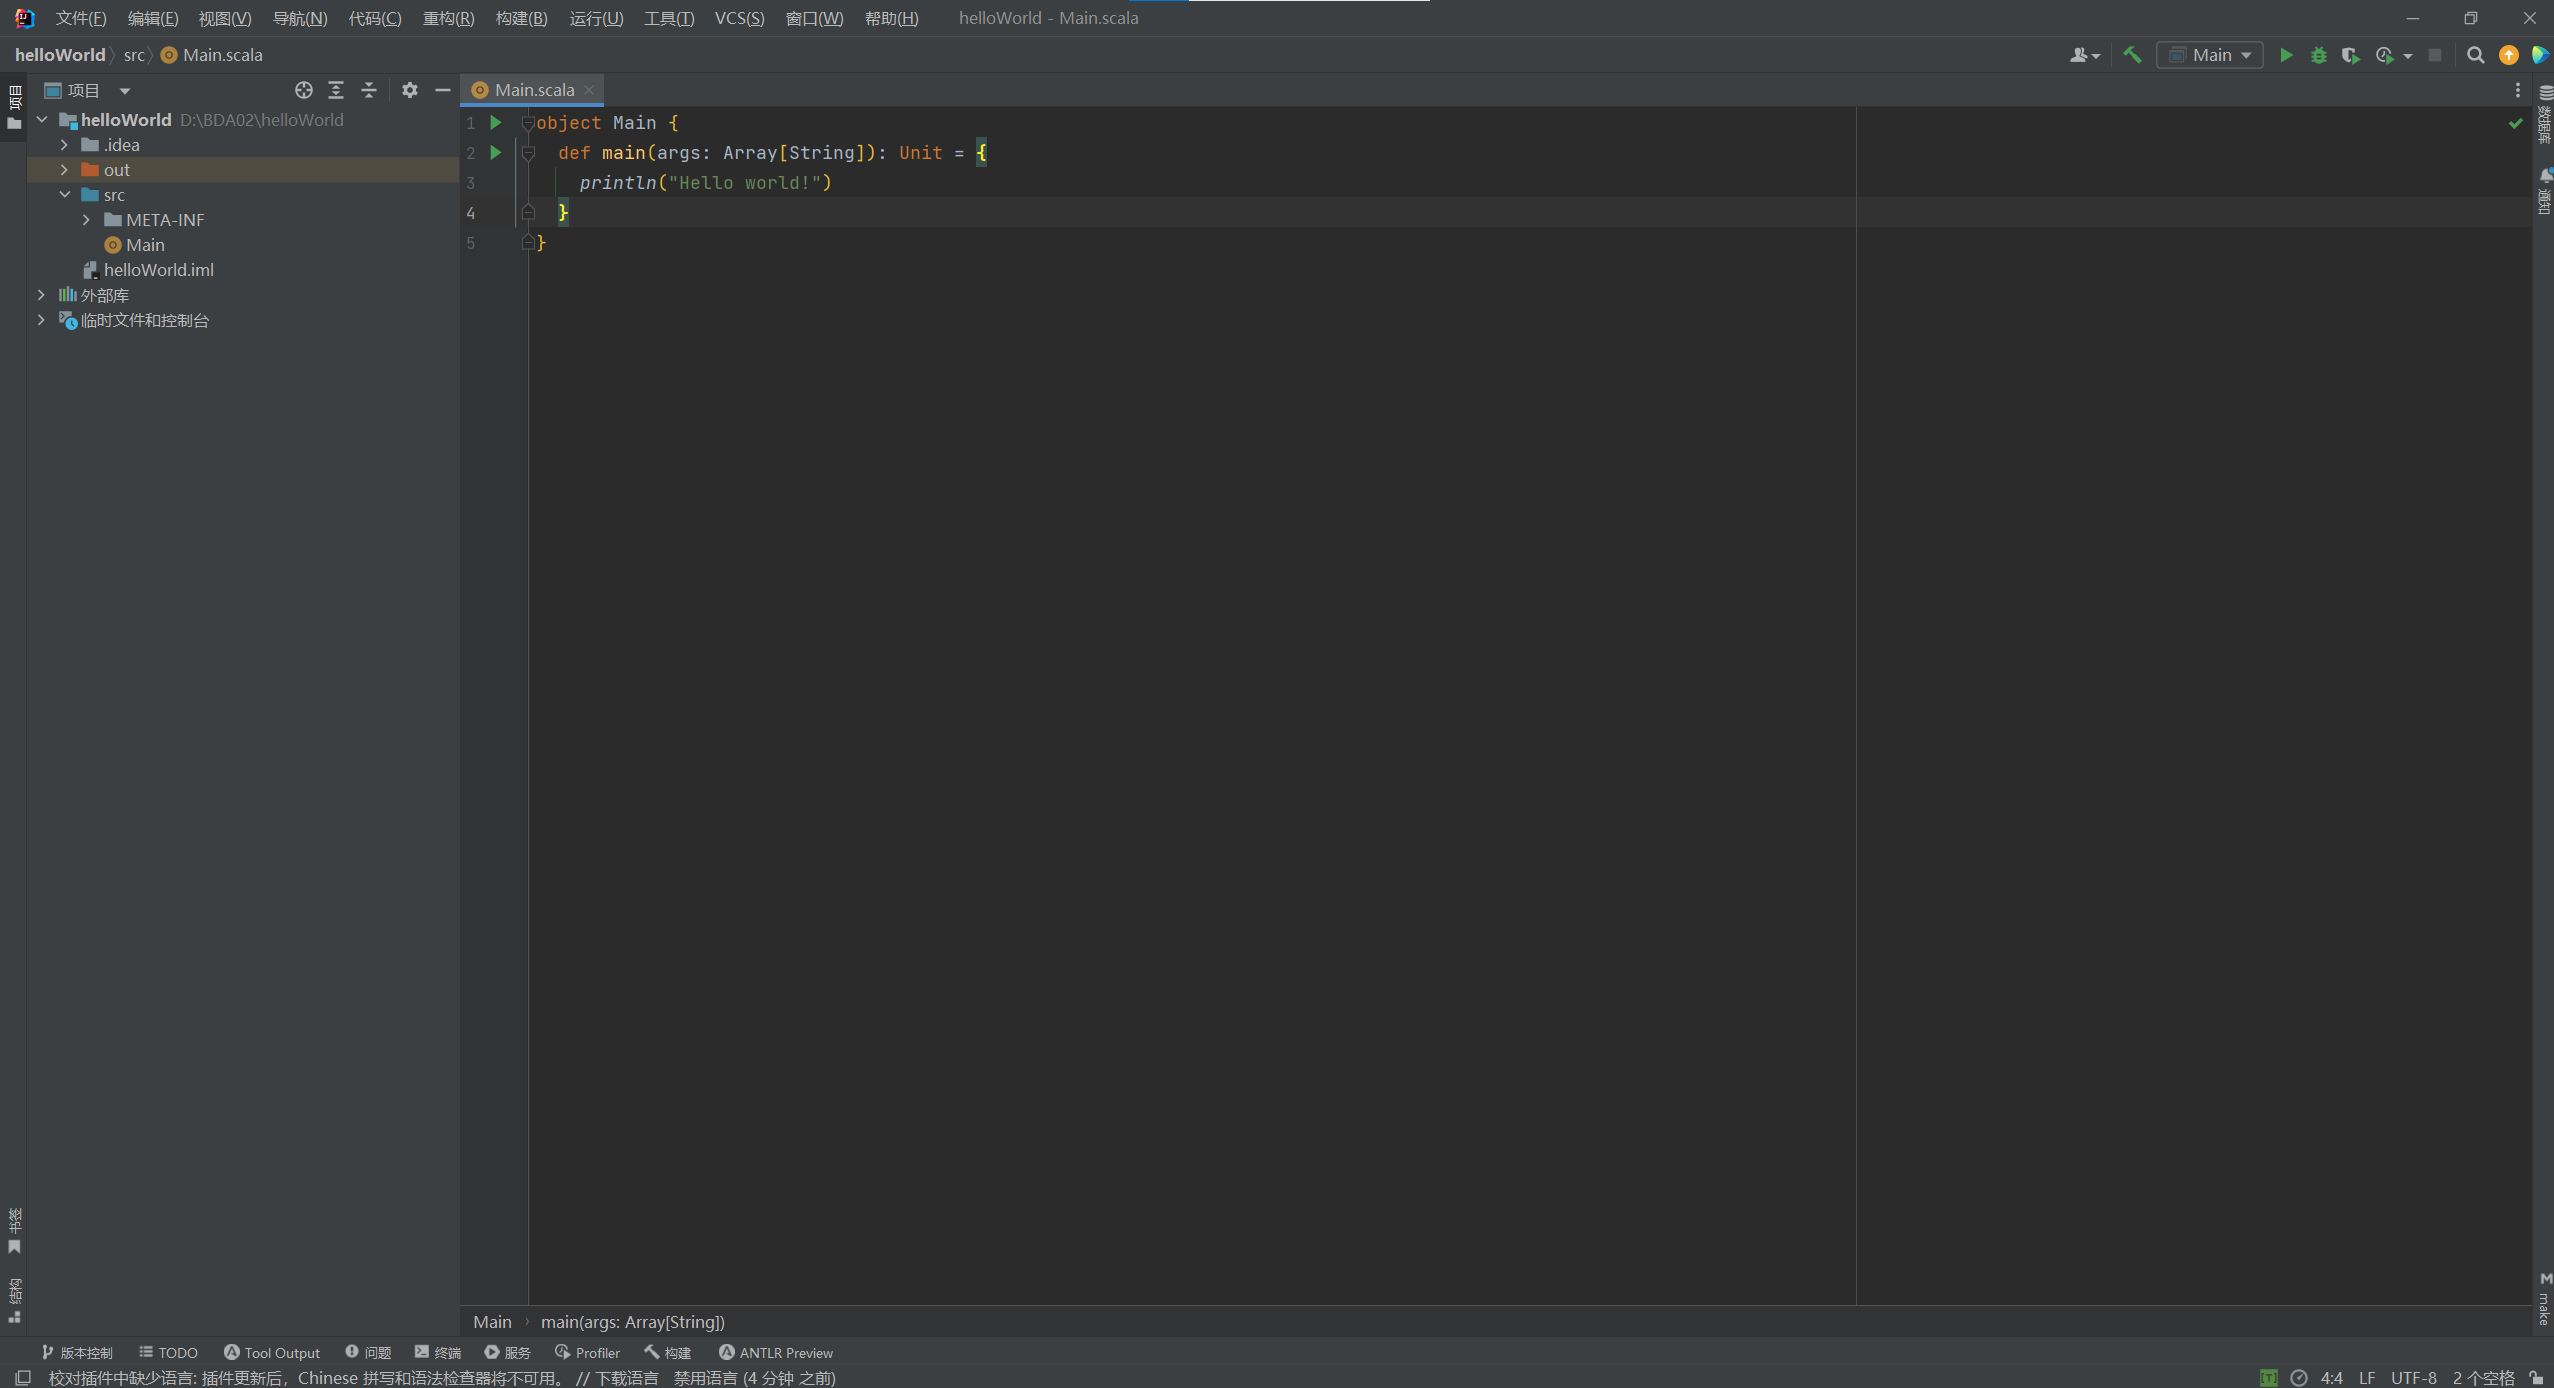
\includegraphics[width=\textwidth]{figure/code.png}
  \caption{hello world程序}
  \label{fig:my_label}
\end{figure}

    
\section{打jar包}
\subsection{使用IDEA将项目打成jar包}
\begin{figure}[H]
  \centering
  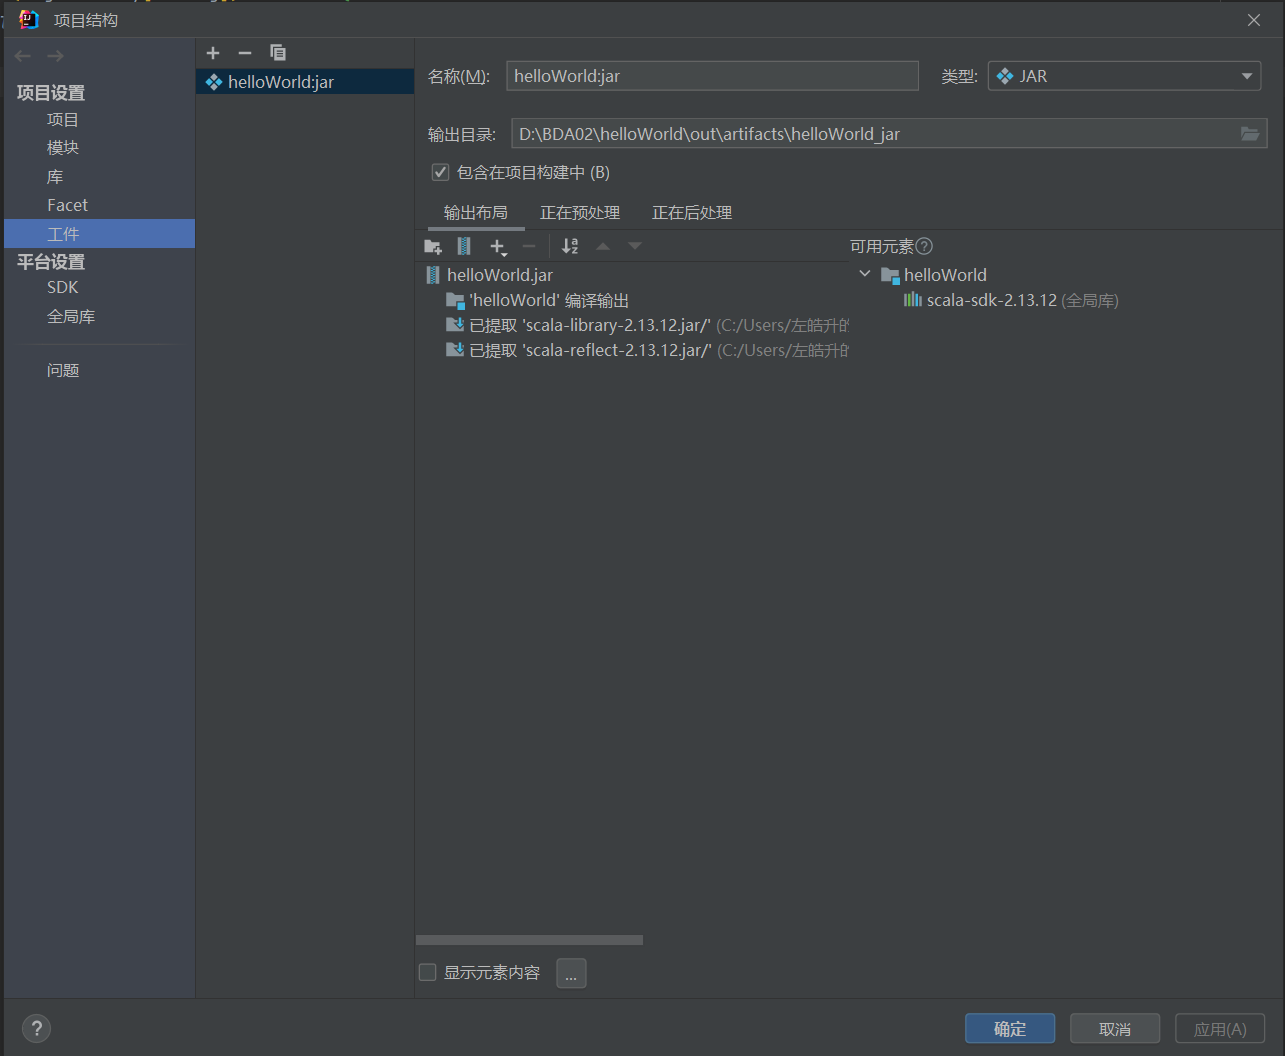
\includegraphics[width=\textwidth]{figure/jar.png}
  \caption{使用IDEA打jar包}
  \label{fig:my_label}
\end{figure}

\subsection{本地测试运行jar包}
\begin{figure}[H]
  \centering
  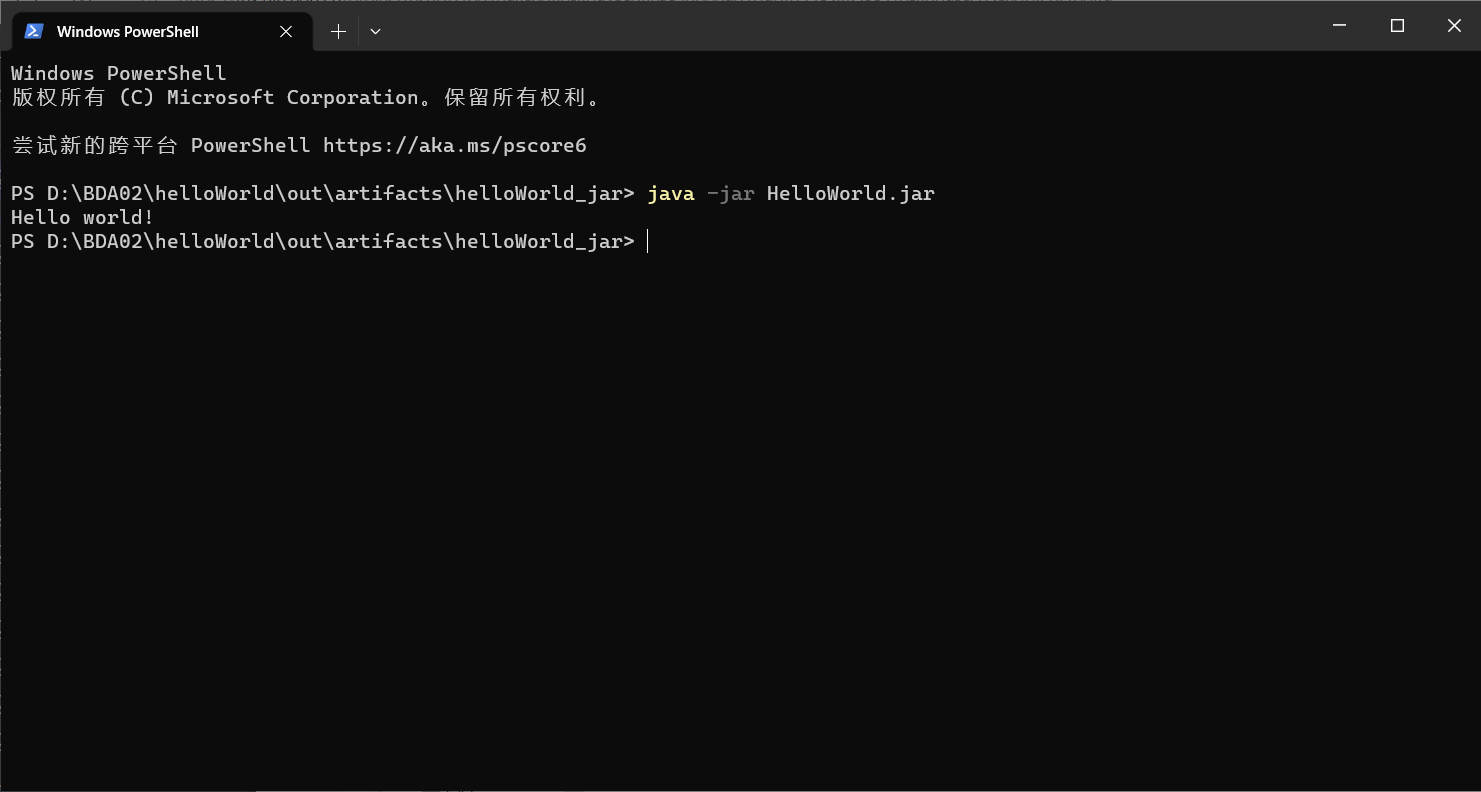
\includegraphics[width=\textwidth]{figure/test.png}
  \caption{本地运行jar包}
  \label{fig:my_label}
\end{figure}

\section{使用阿里云搭建EMR on ECS服务器}
\subsection{配置搭建过程}
\begin{figure}[H]
  \centering
  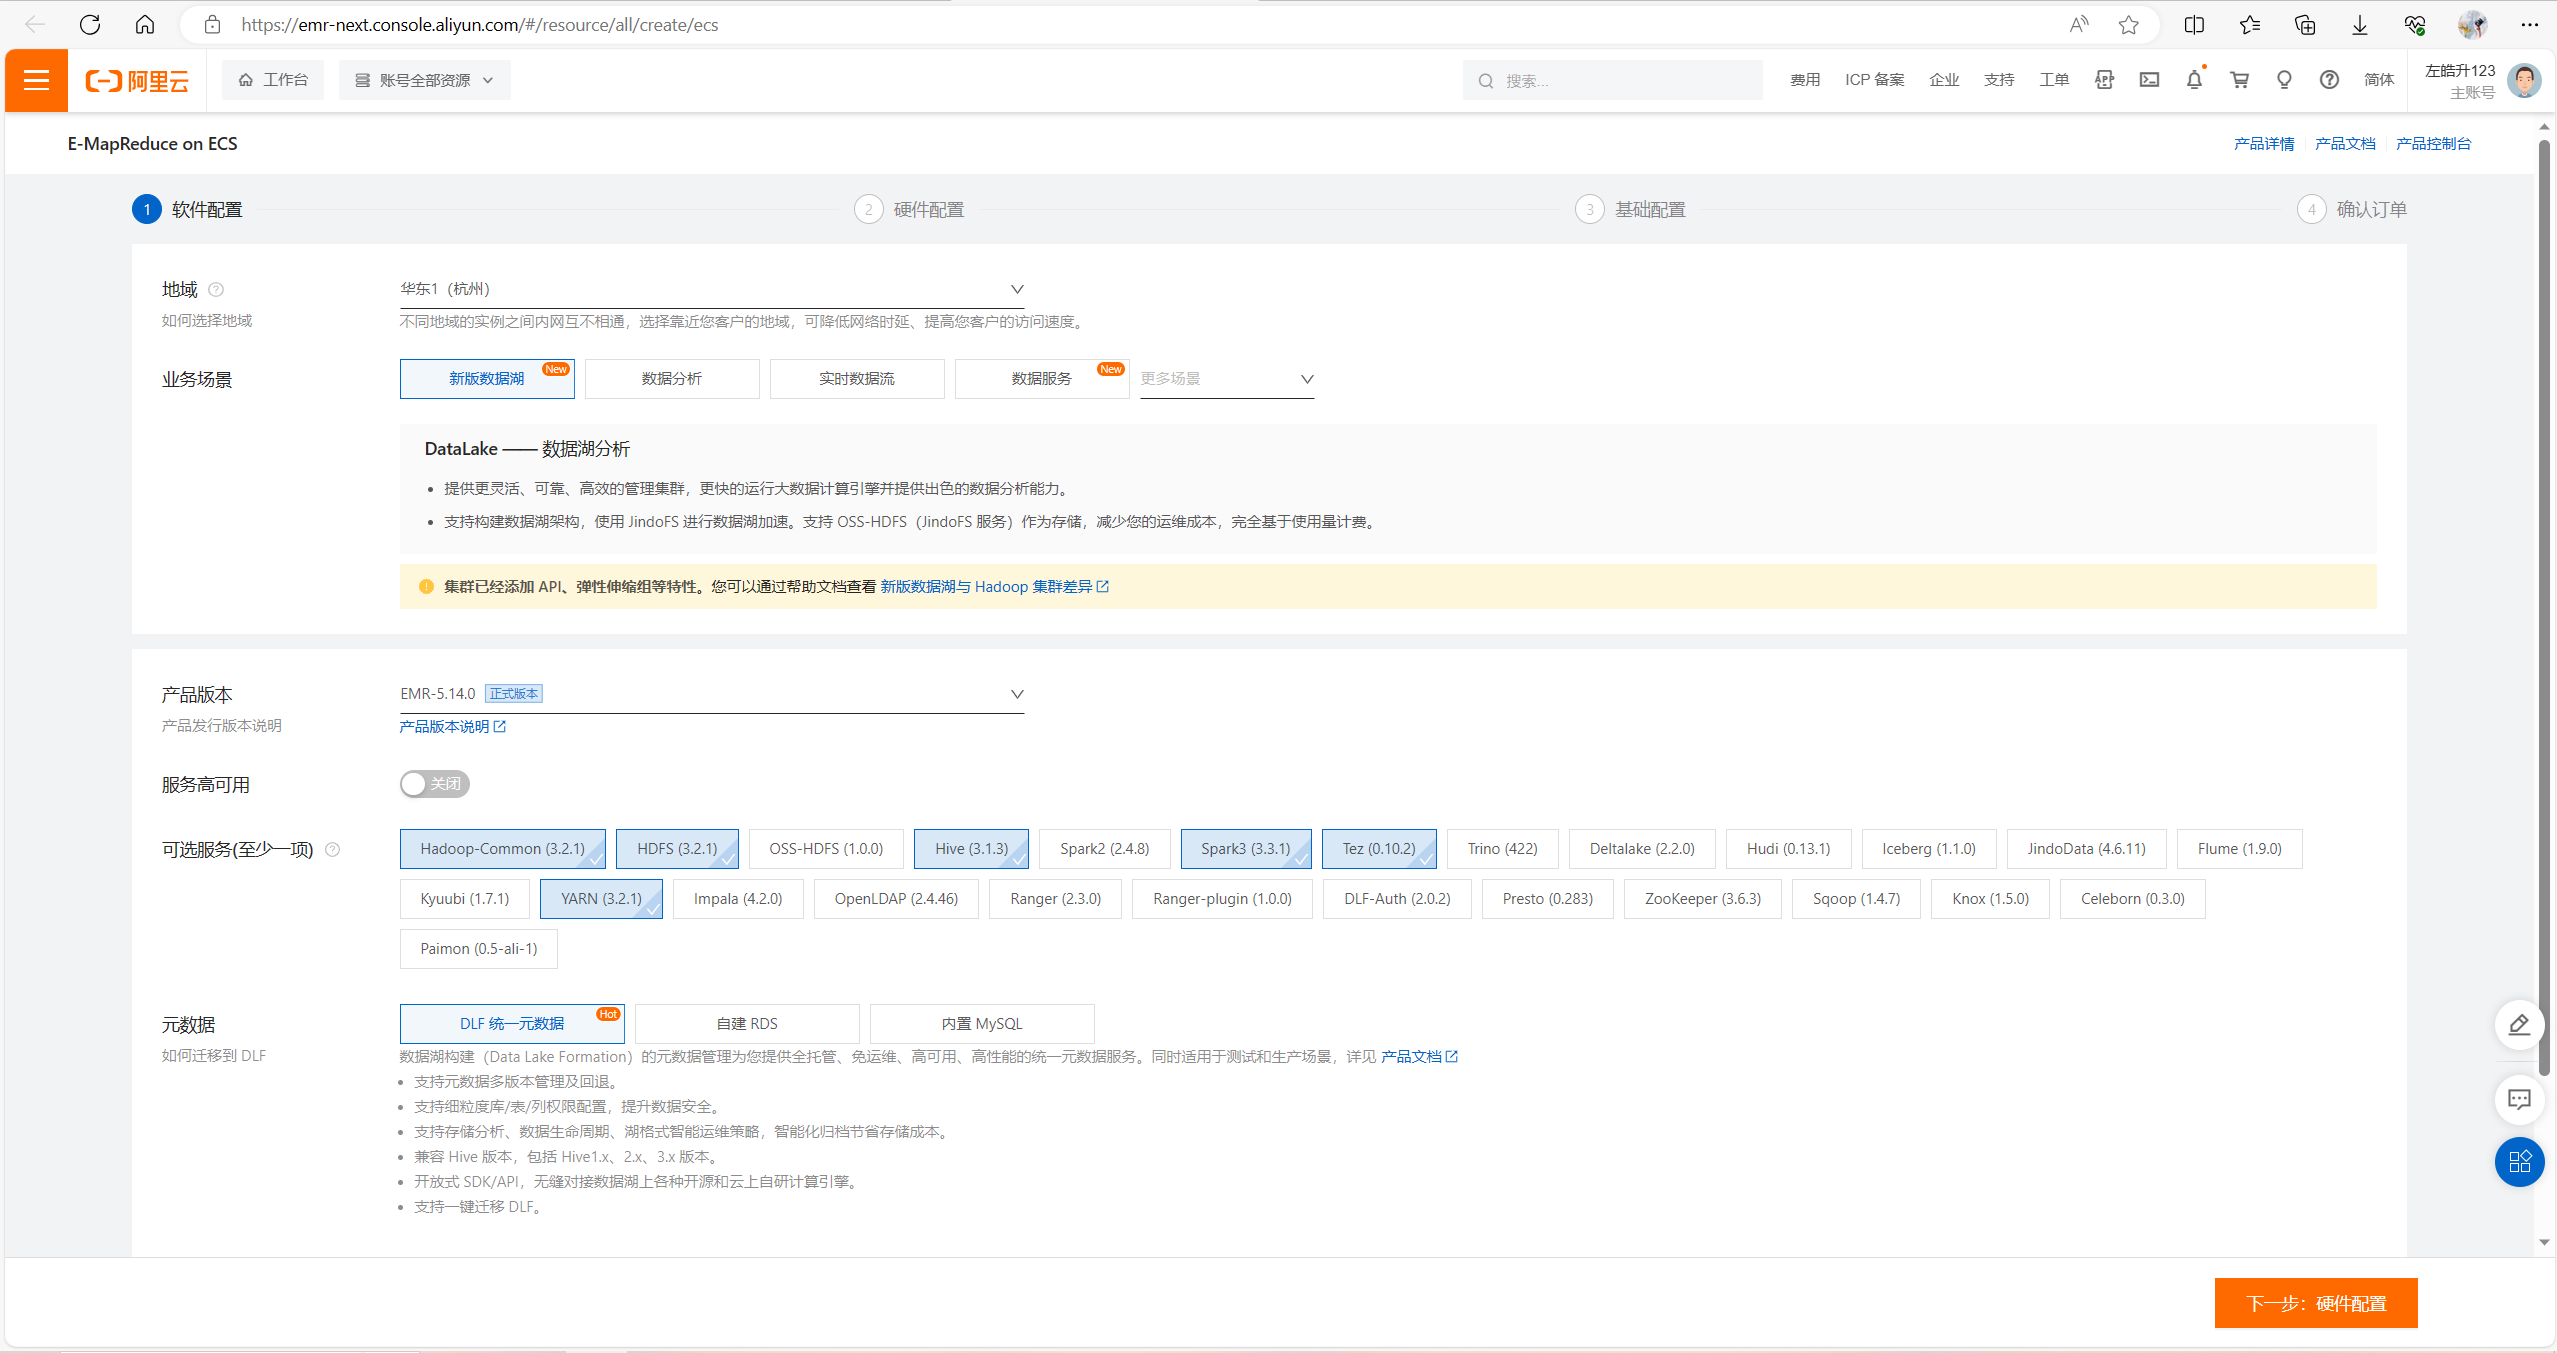
\includegraphics[width=\textwidth]{figure/setting1.png}
  \caption{选择需要的服务}
  \label{fig:my_label}
\end{figure}
\begin{figure}[H]
  \centering
  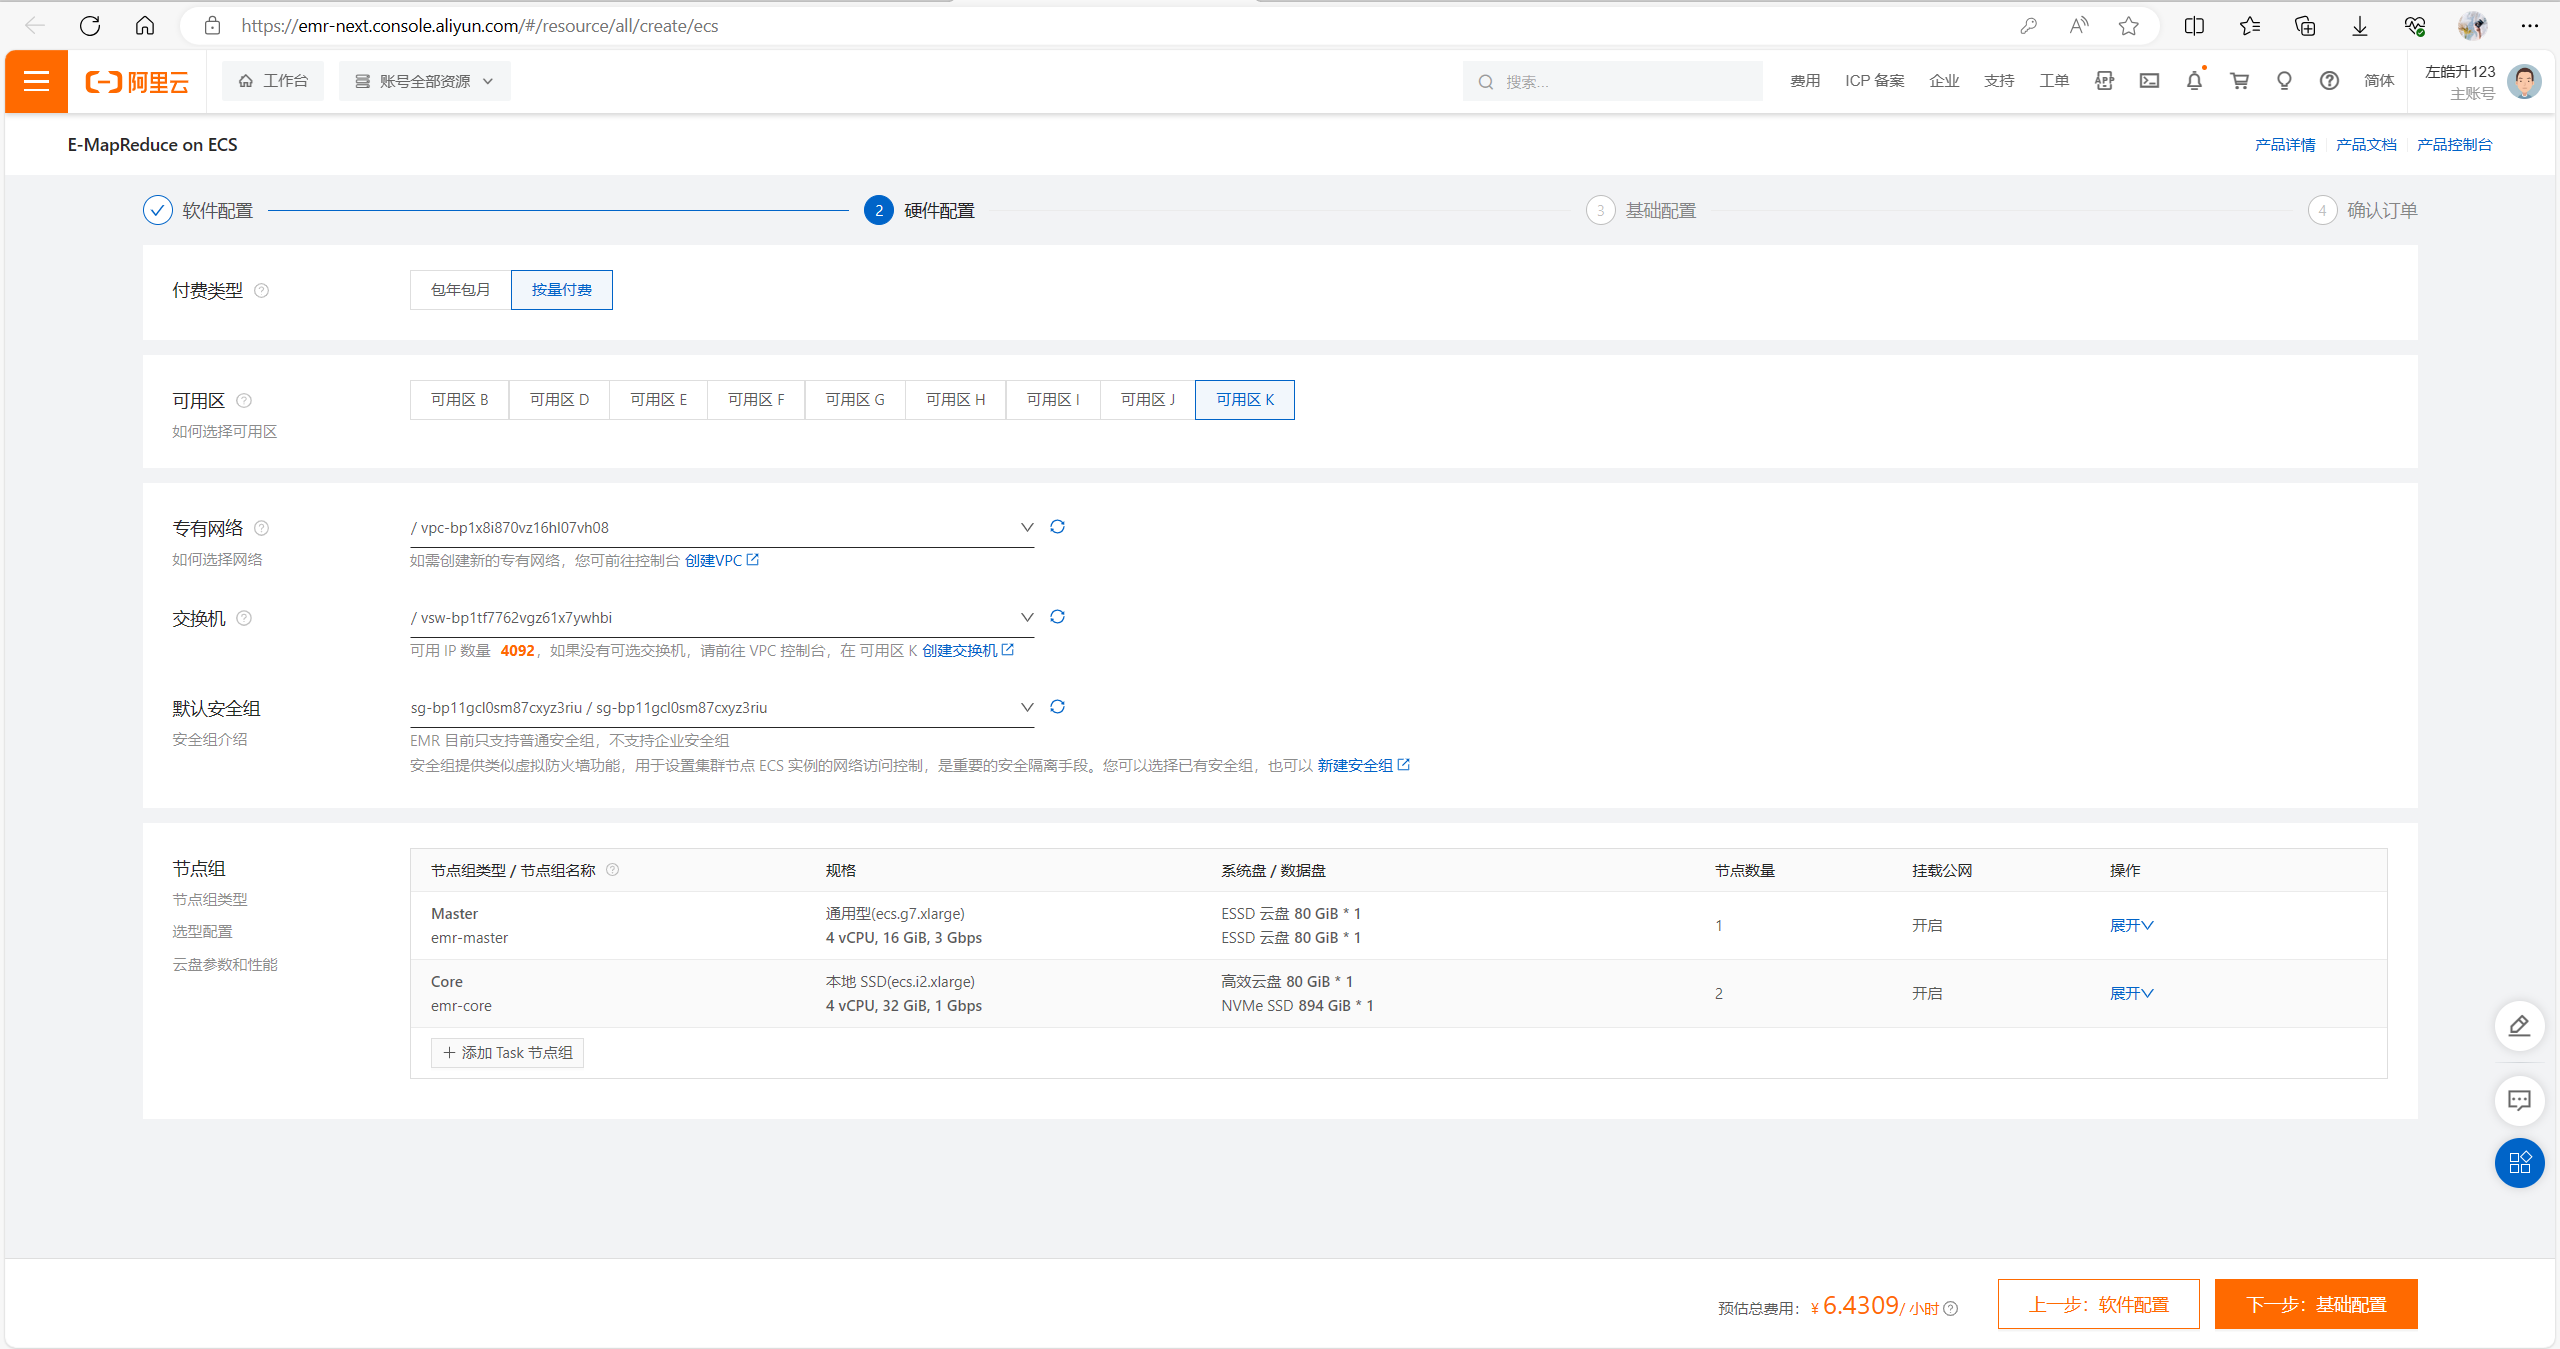
\includegraphics[width=\textwidth]{figure/setting2.png}
  \caption{配置交换机,设置公网IP便于SSH访问}
  \label{fig:my_label}
\end{figure}
\begin{figure}[H]
  \centering
  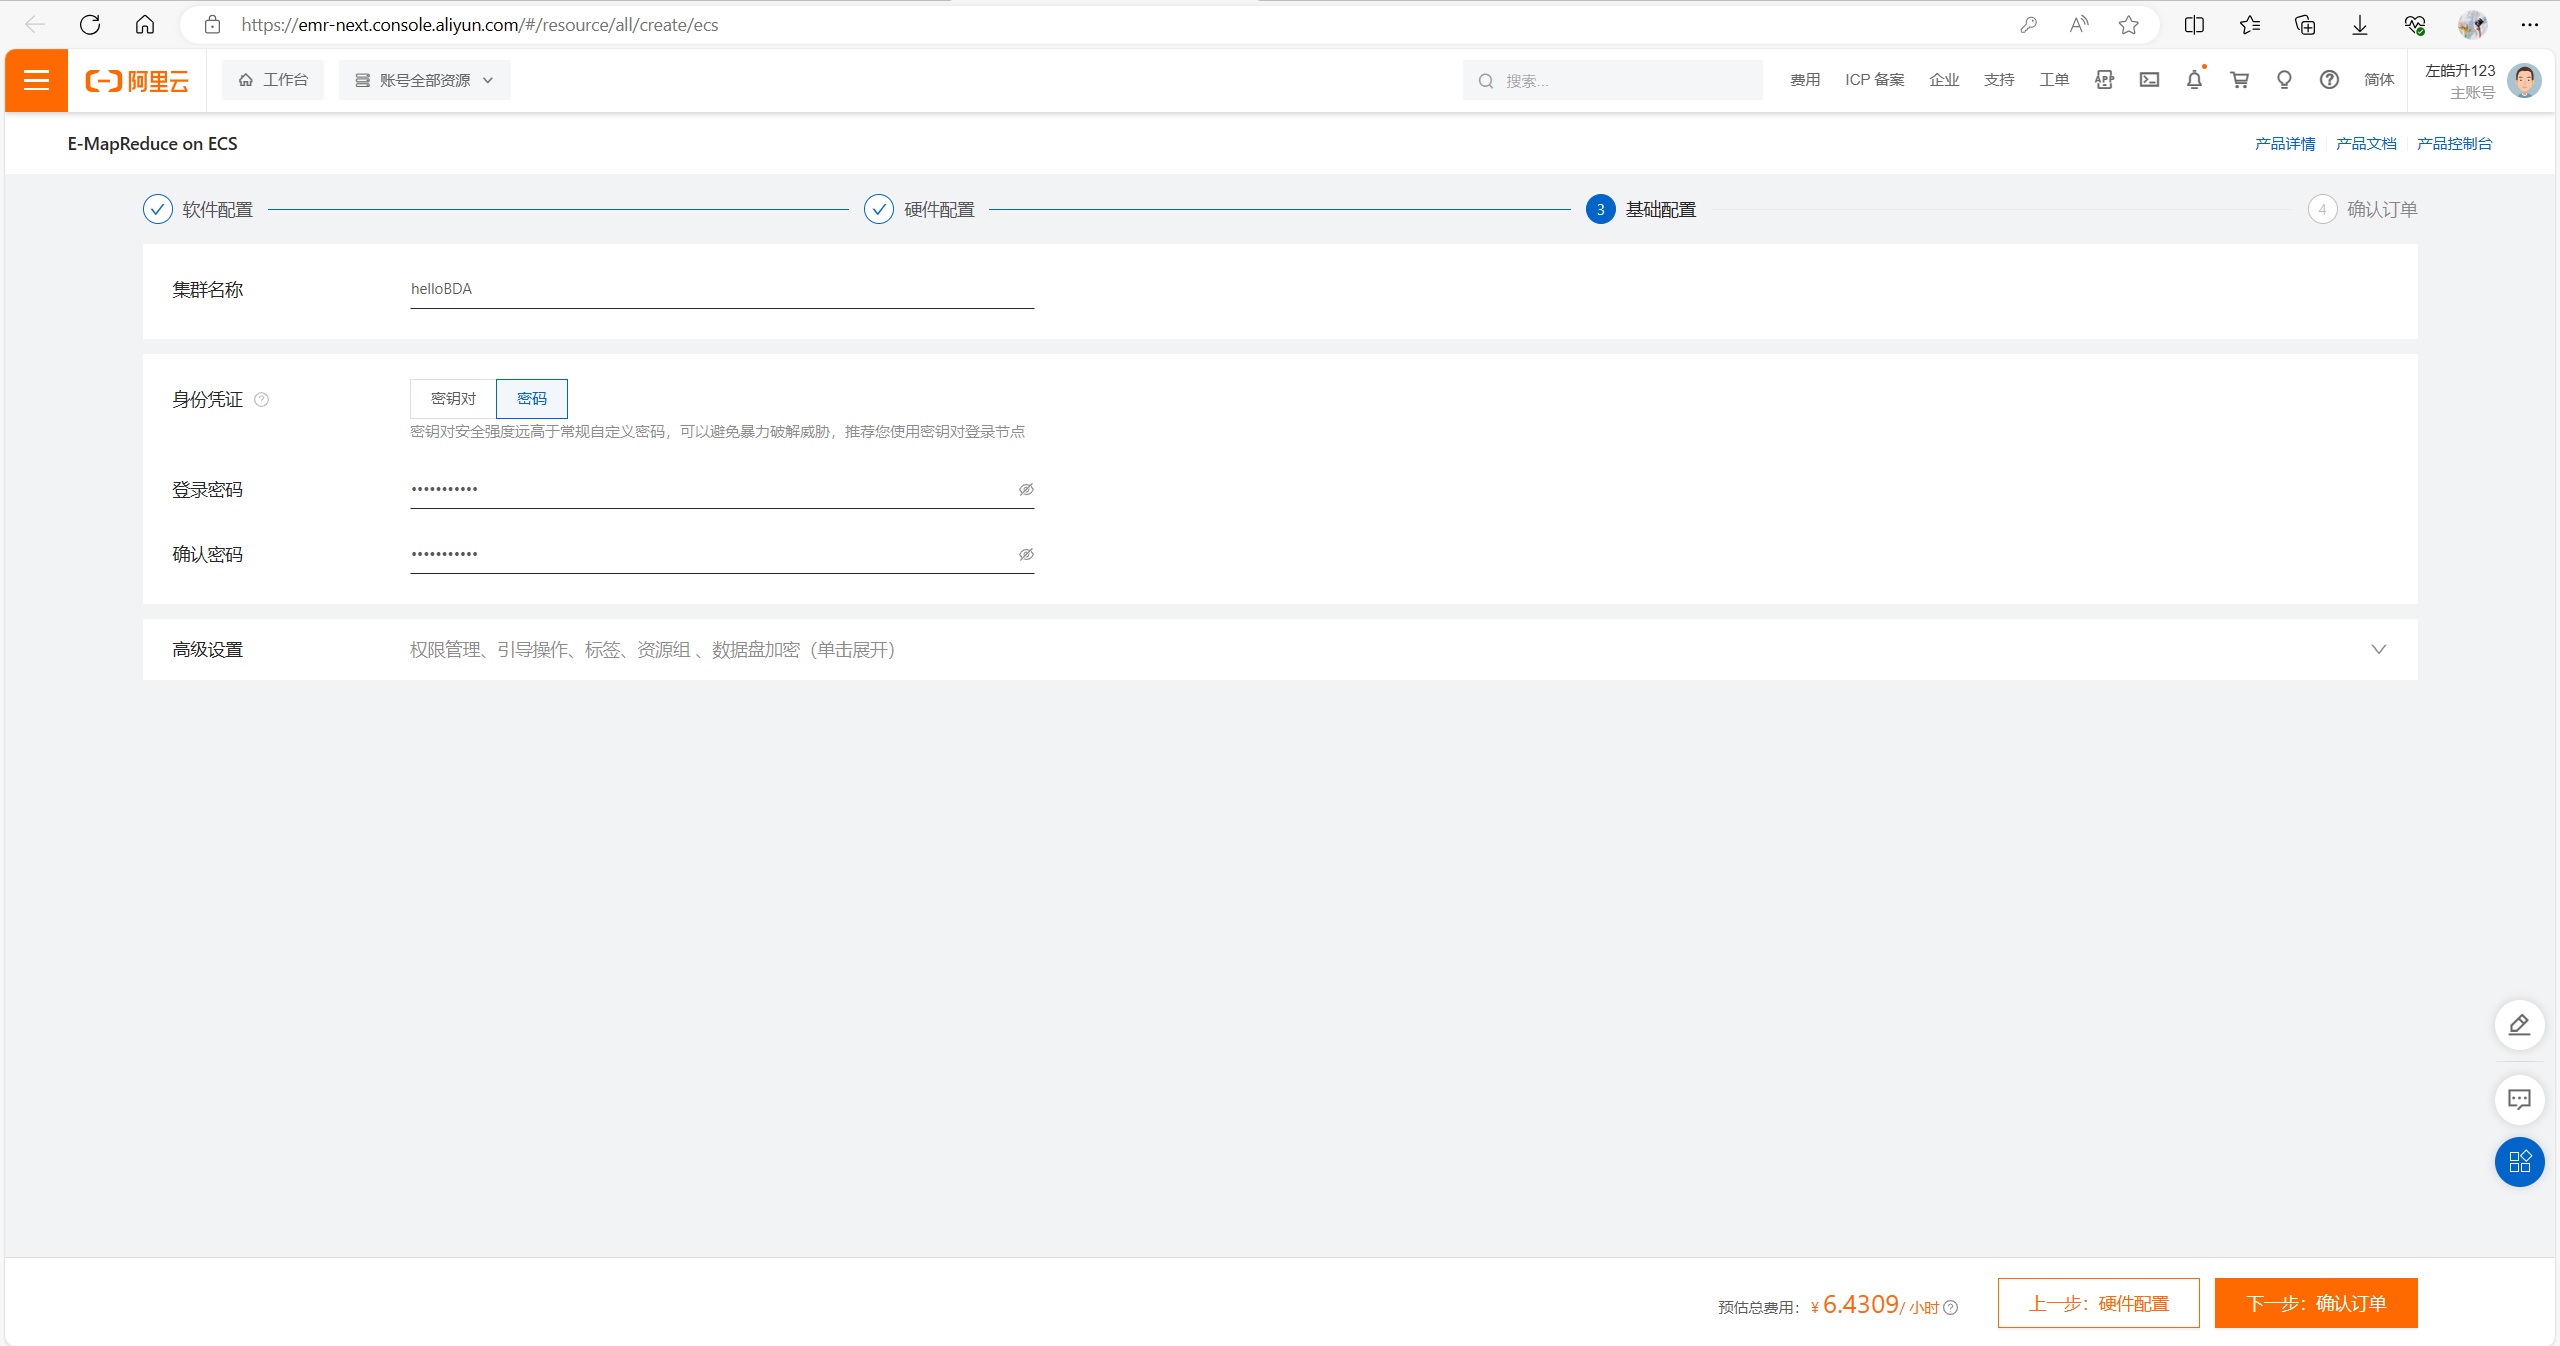
\includegraphics[width=\textwidth]{figure/setting3.png}
  \caption{设置密码}
  \label{fig:my_label}
\end{figure}
\begin{figure}[H]
  \centering
  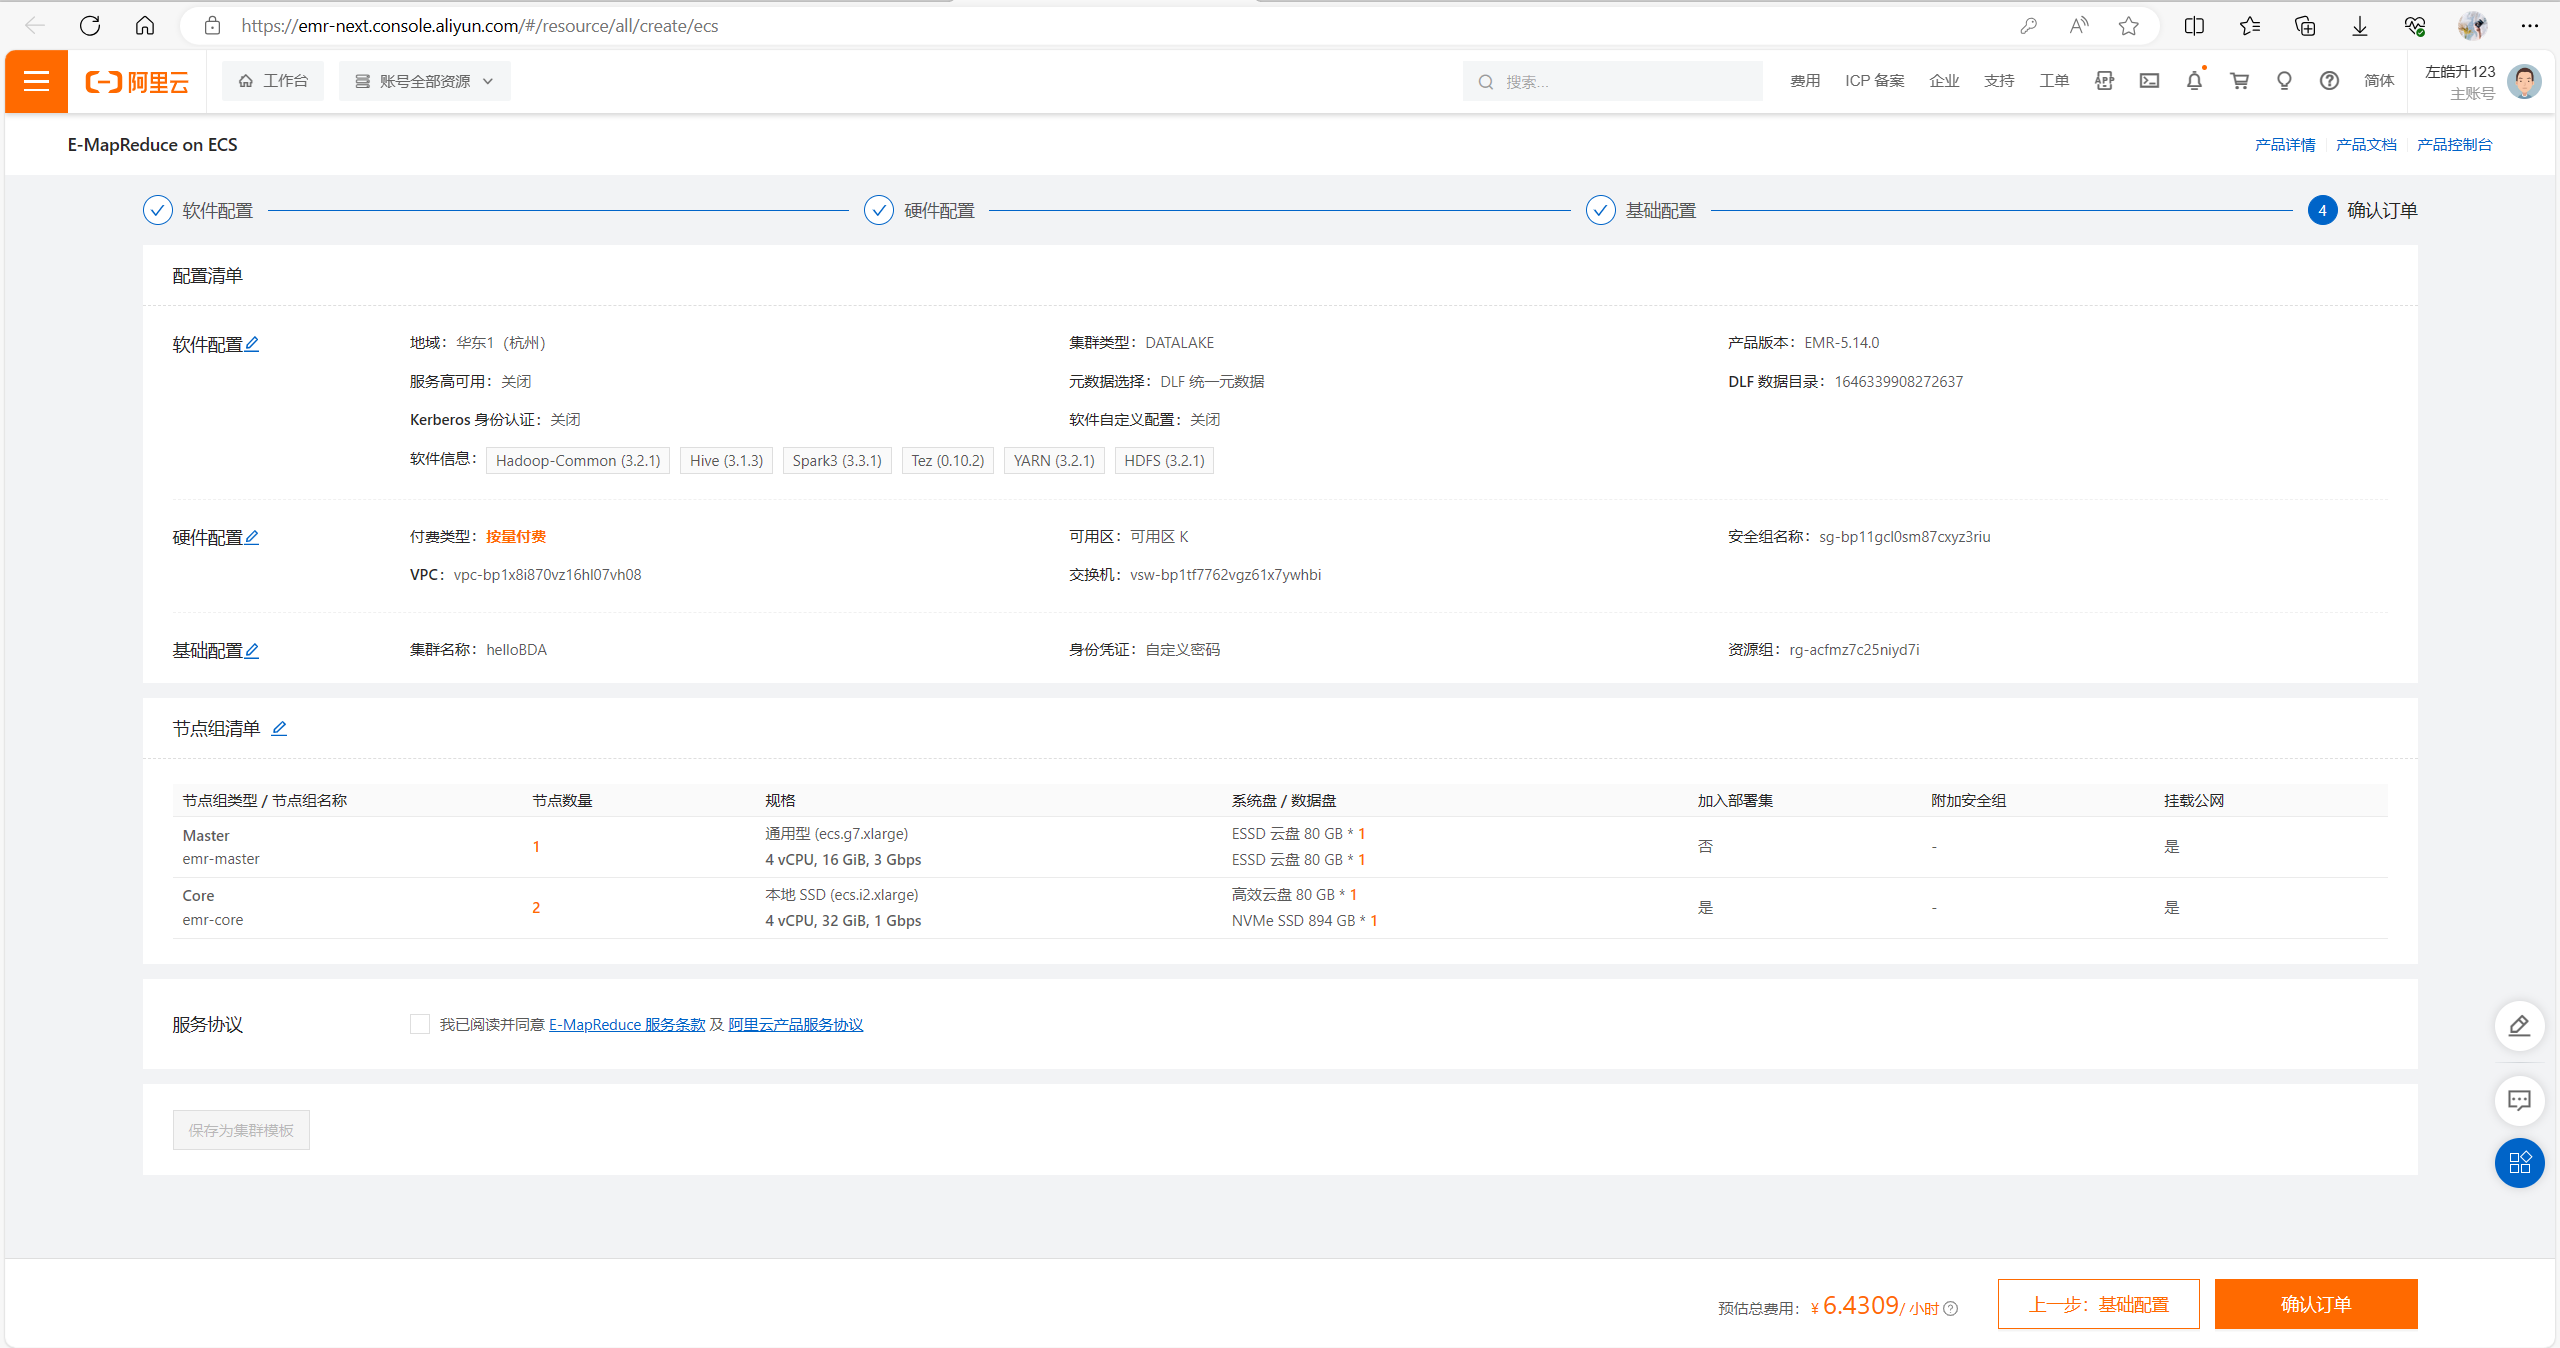
\includegraphics[width=\textwidth]{figure/setting4.png}
  \caption{服务器配置}
  \label{fig:my_label}
\end{figure}

\subsection{进入工作台,可以看到服务器已经搭建成功,在实例中也可以看到}
\begin{figure}[H]
  \centering
  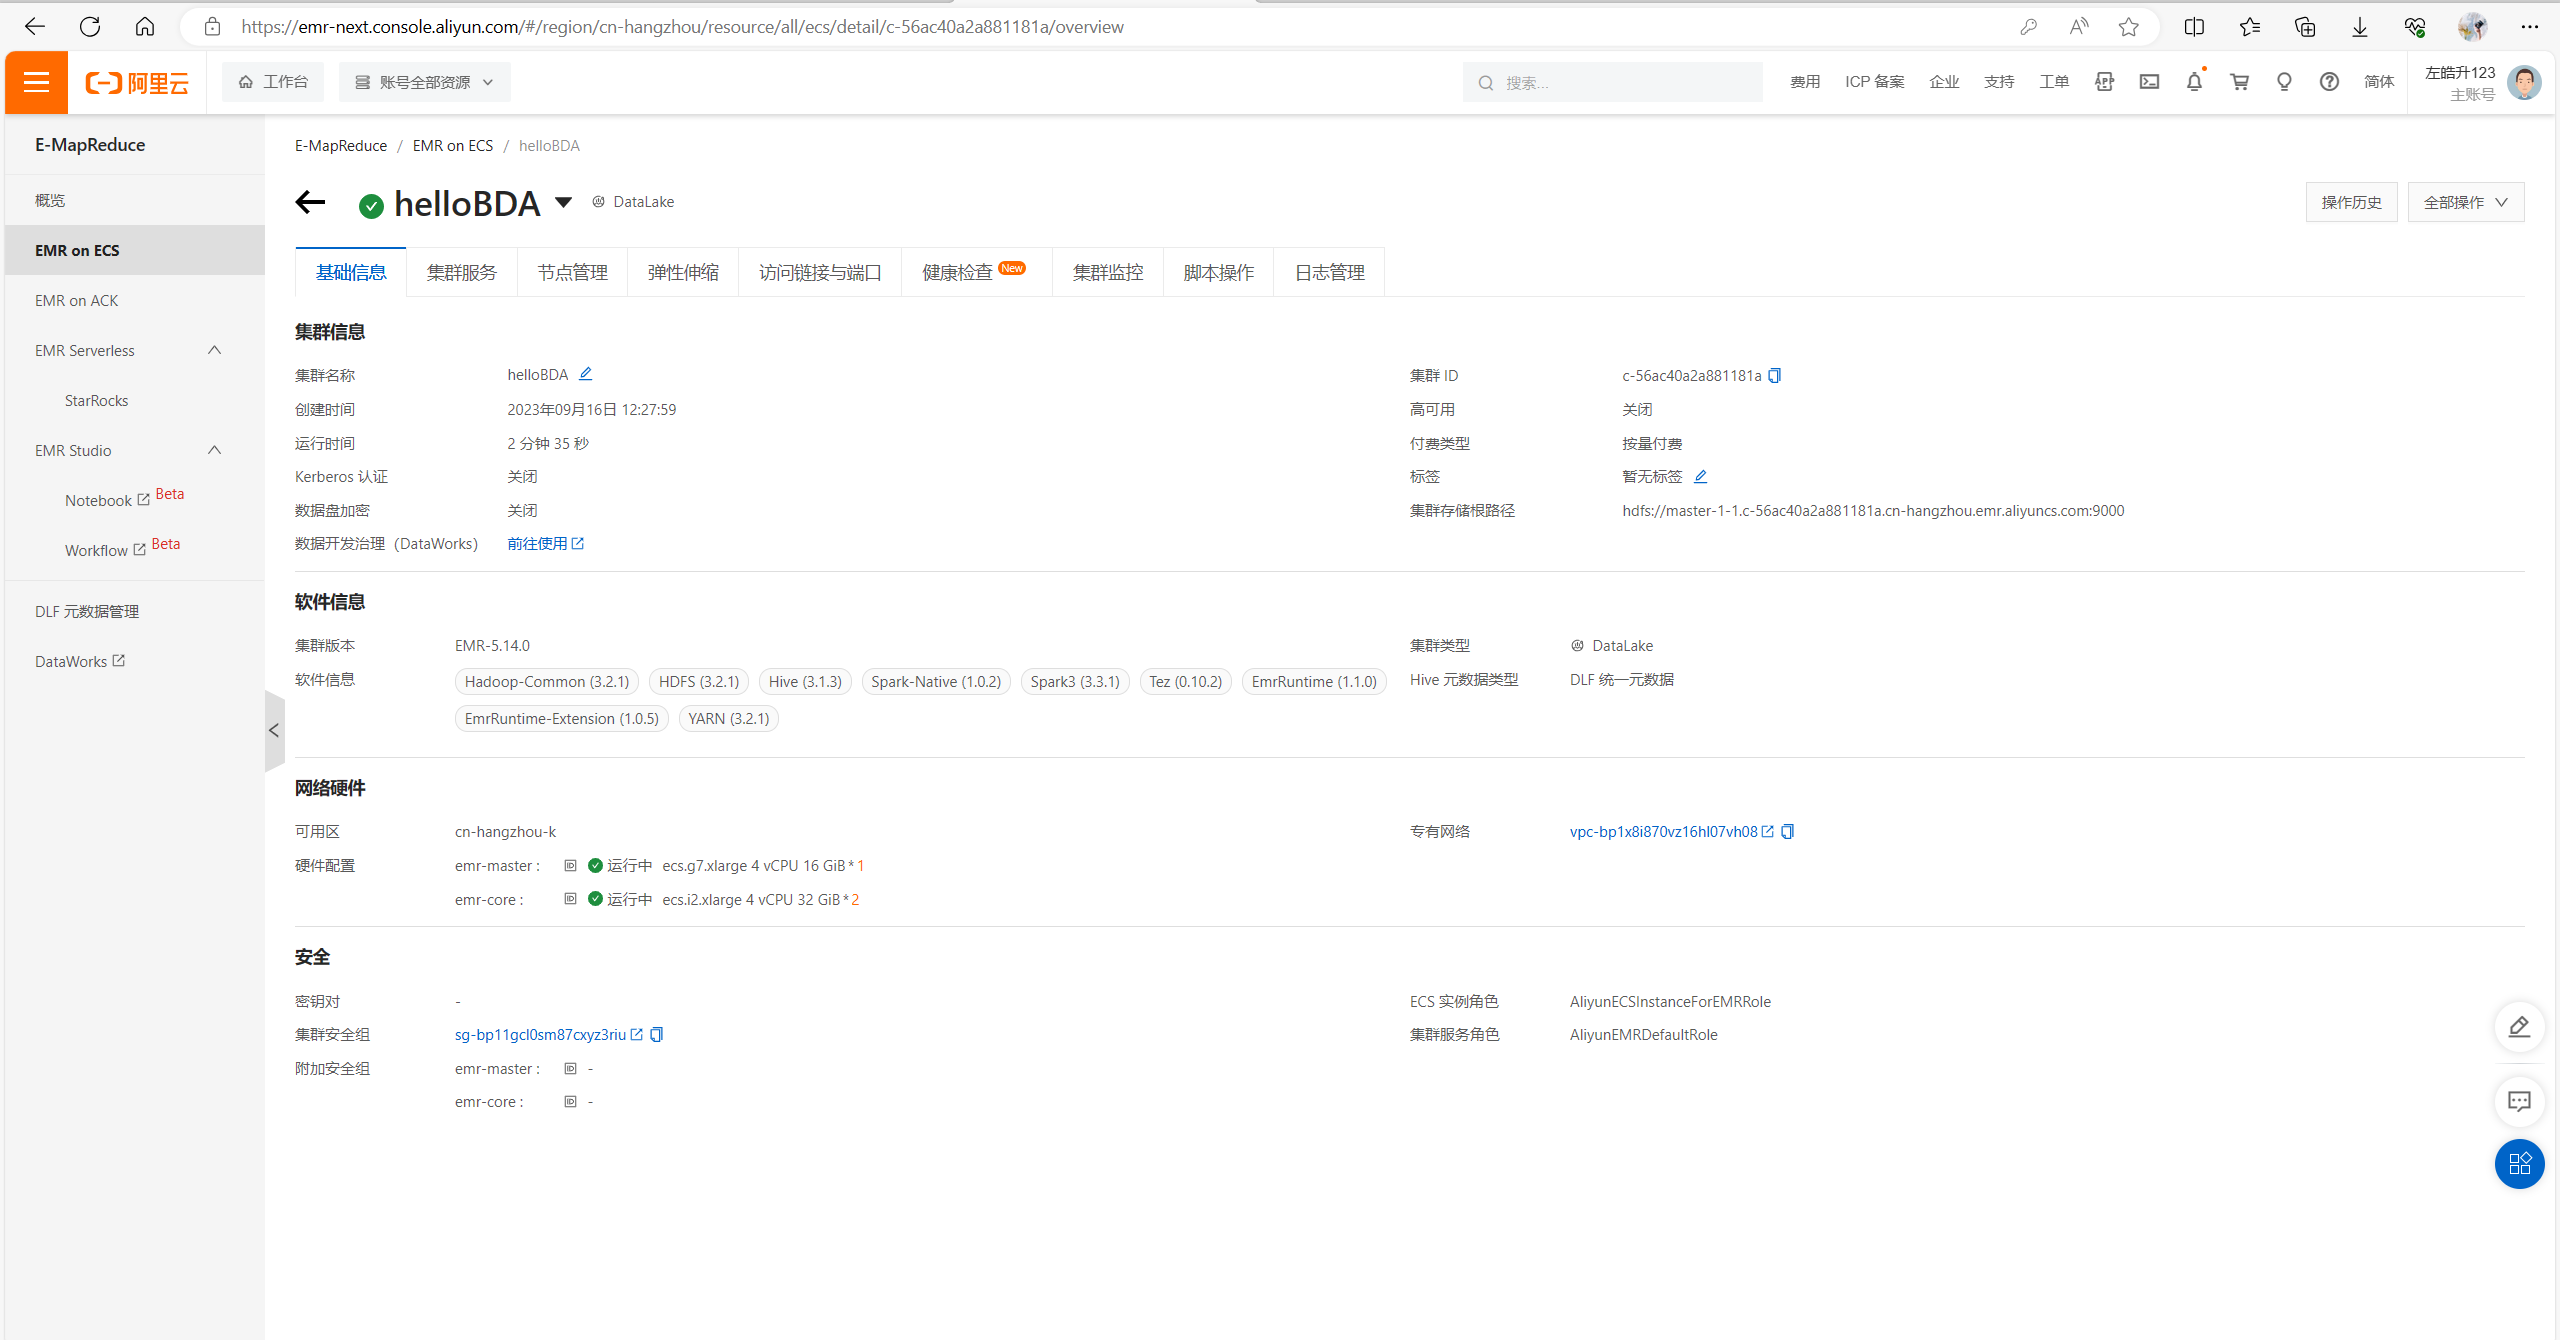
\includegraphics[width=\textwidth]{figure/controller1.png}
  \caption{工作台}
  \label{fig:my_label}
\end{figure}
\begin{figure}[H]
  \centering
  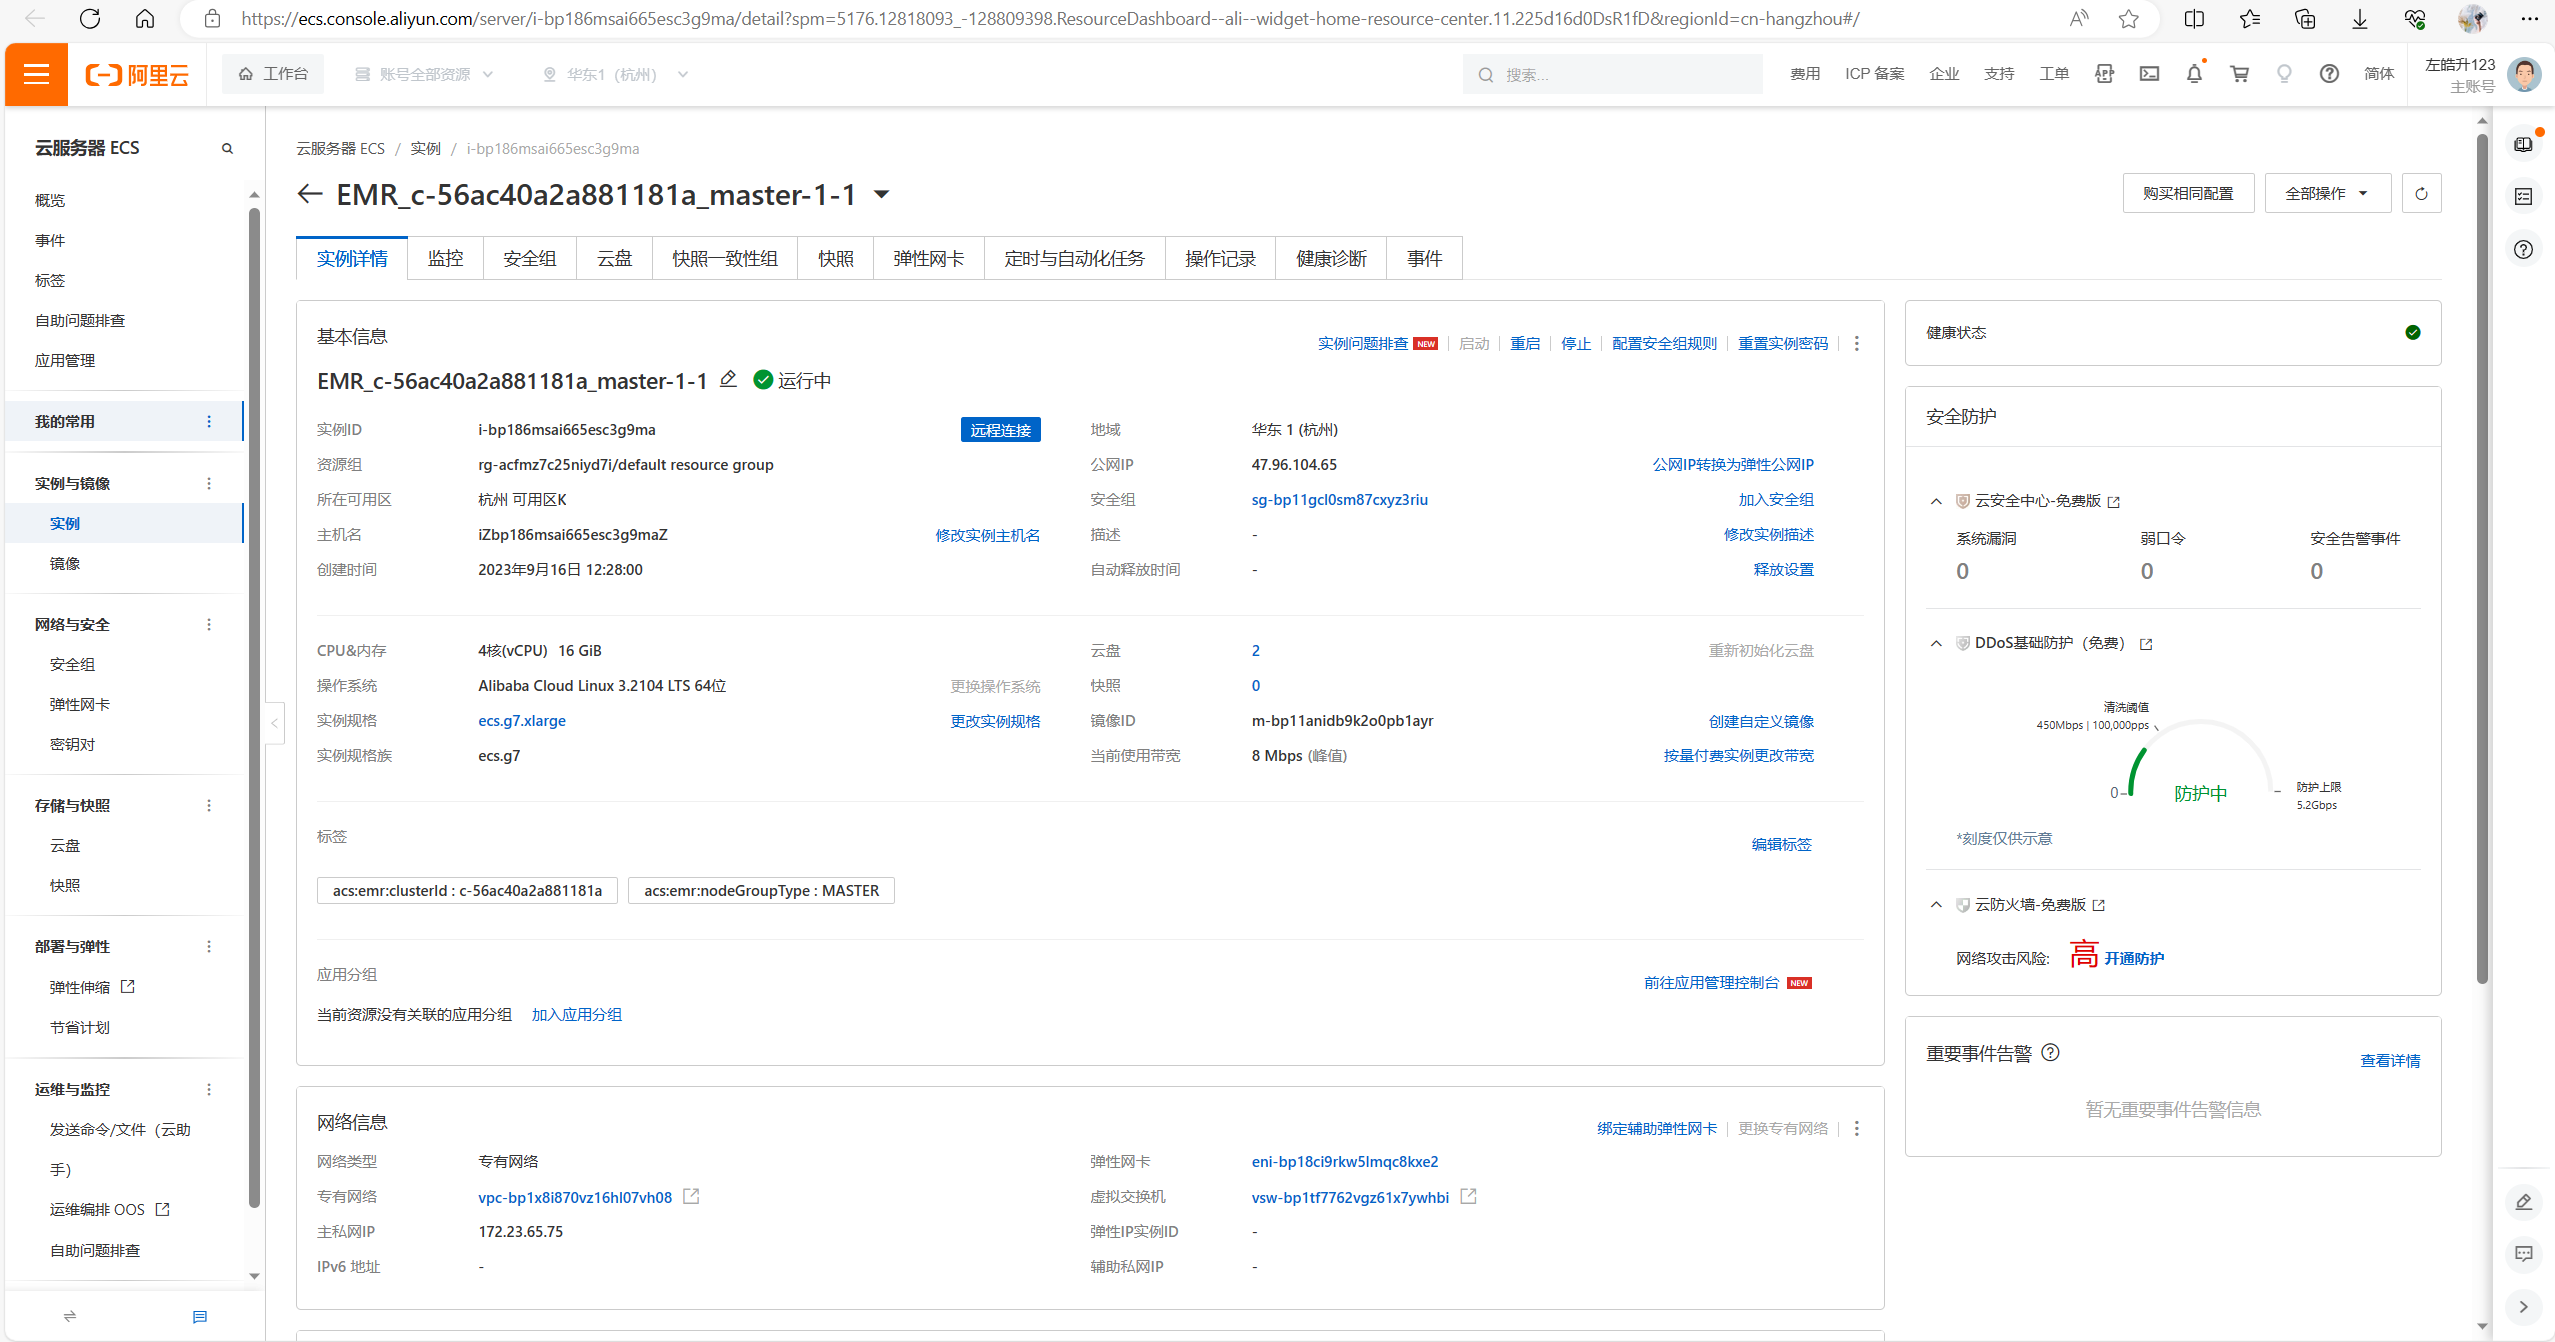
\includegraphics[width=\textwidth]{figure/controller2.png}
  \caption{实例}
  \label{fig:my_label}
\end{figure}


\section{环境测试}
使用ssh连接服务器,并测试spark环境
\begin{figure}[H]
  \centering
  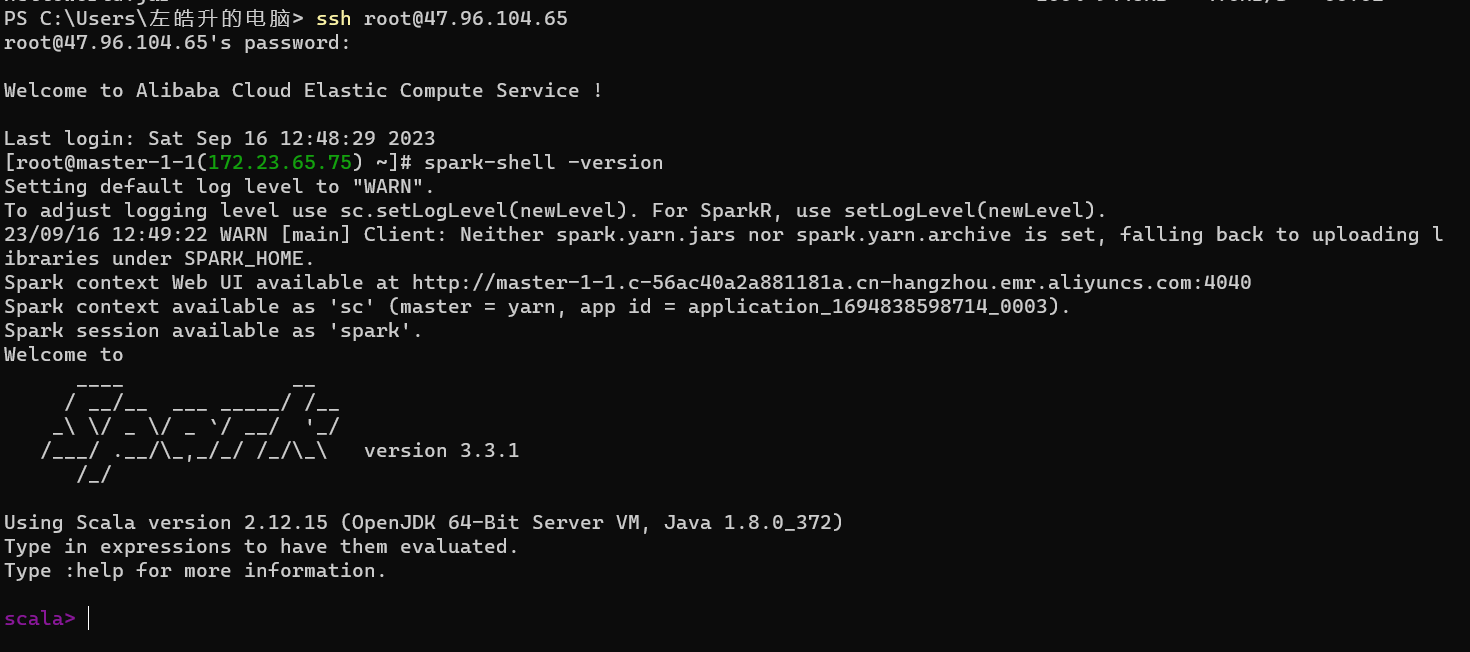
\includegraphics[width=\textwidth]{figure/ssh.png}
  \caption{实例}
  \label{fig:my_label}
\end{figure}

\section{运行程序}
\subsection{使用scp将本地的jar包上传}
\begin{figure}[H]
  \centering
  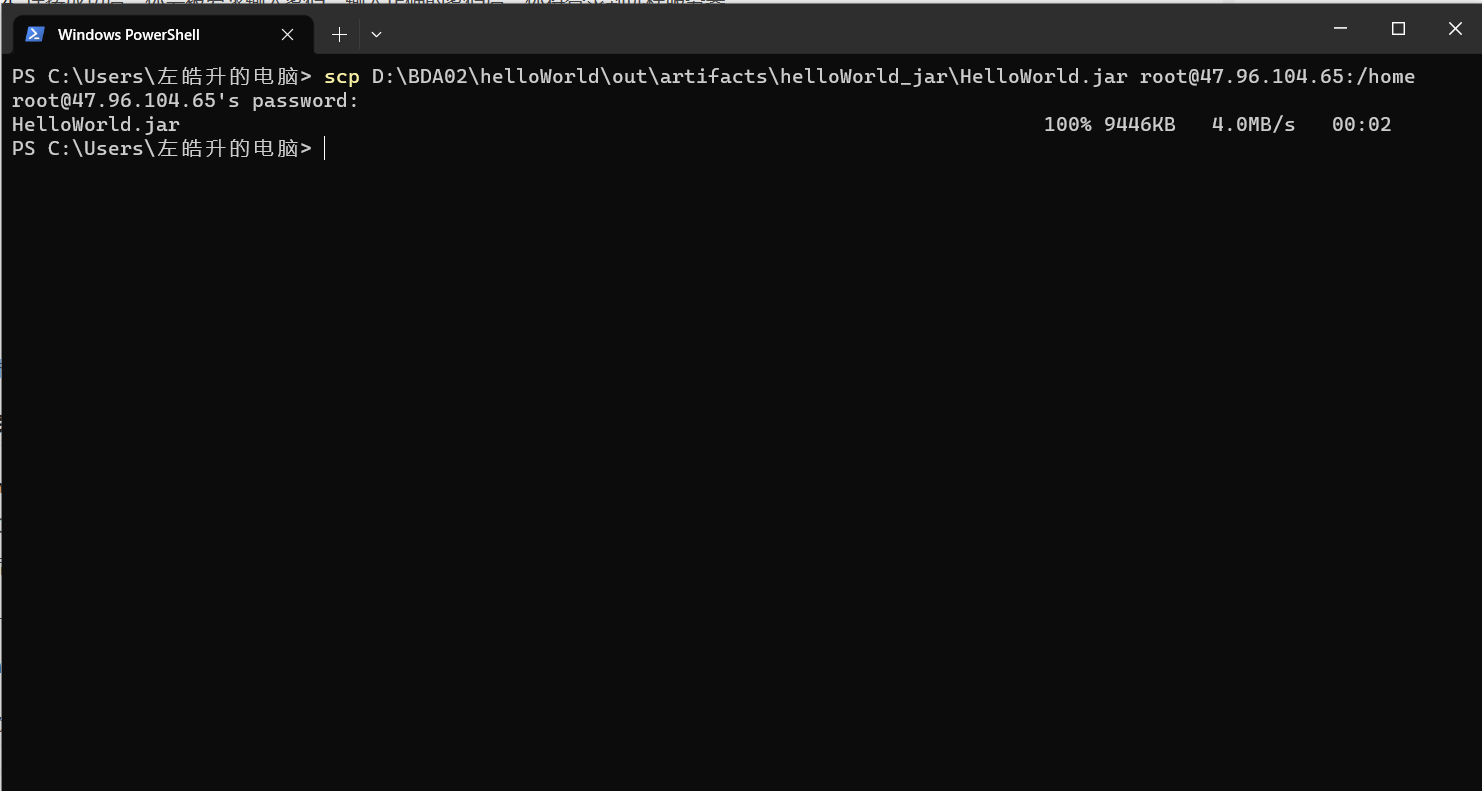
\includegraphics[width=\textwidth]{figure/scp.png}
  \caption{实例}
  \label{fig:my_label}
\end{figure}

\subsection{运行jar包}
\begin{figure}[H]
  \centering
  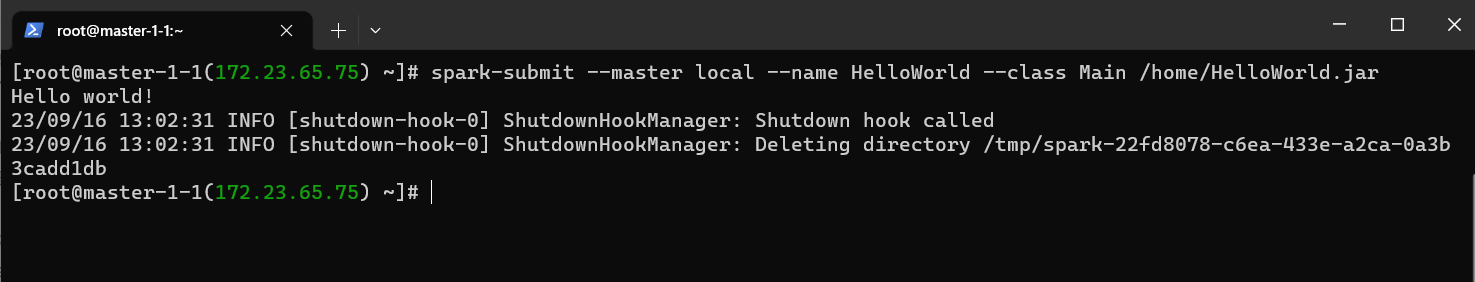
\includegraphics[width=\textwidth]{figure/run.png}
  \caption{实例}
  \label{fig:my_label}
\end{figure}
成功输出了Hello, World!

\section{挑战以及克服}
\subsection{选用什么样的云服务}
一开始不知道应该使用什么样的云服务,尝试了微软的Azure,阿里云ECS,最终结合自己对作业要求的理解以及作业中对amazon EMR的推荐,选择了阿里云的EMR。
\subsection{如何配置EMR}
以前没有接触过大数据和云服务器,在配置过程中不知道自己需要什么样的服务,对于配置中给出的各种名词也不了解,不知道应该做出什么样的选择,交换机该如何配置。在配置过程中,遇到不认识的就去bing上搜索,去了解,大概知道这是什么东西,起着什么样的作用。
\subsection{如何在EMR上运行代码}
一开始不知道如何在服务器上运行代码,直接把代码传上去却发现没法运行。后来去搜索才知道,运行jar包是一个更好的选择。于是使用IDEA先打好jar包再传上去运行。